\documentclass[12pt]{scrartcl}


\setlength{\parindent}{0pt}
\setlength{\parskip}{.25cm}

\usepackage{graphicx}

\usepackage{xcolor}

\definecolor{darkred}{rgb}{0.5,0,0}
\definecolor{darkgreen}{rgb}{0,0.5,0}
\usepackage{hyperref}
\hypersetup{
  letterpaper,
  colorlinks,
  linkcolor=red,
  citecolor=darkgreen,
  menucolor=darkred,
  urlcolor=blue,
  pdfpagemode=none,
  pdftitle={Introduction To Git},
  pdfauthor={Christopher M. Bourke},
  pdfcreator={$ $Id: cv-us.tex,v 1.28 2009/01/01 00:00:00 cbourke Exp $ $},
  pdfsubject={PhD Thesis},
  pdfkeywords={}
}

\definecolor{MyDarkBlue}{rgb}{0,0.08,0.45}
\definecolor{MyDarkRed}{rgb}{0.45,0.08,0}
\definecolor{MyDarkGreen}{rgb}{0.08,0.45,0.08}

\definecolor{mintedBackground}{rgb}{0.95,0.95,0.95}
\definecolor{mintedInlineBackground}{rgb}{.90,.90,1}

%\usepackage{newfloat}
\usepackage[newfloat=true]{minted}
\setminted{mathescape,
               linenos,
               autogobble,
               frame=none,
               framesep=2mm,
               framerule=0.4pt,
               %label=foo,
               xleftmargin=2em,
               xrightmargin=0em,
               startinline=true,  %PHP only, allow it to omit the PHP Tags *** with this option, variables using dollar sign in comments are treated as latex math
               numbersep=10pt, %gap between line numbers and start of line
               style=default, %syntax highlighting style, default is "default"
               			    %gallery: http://help.farbox.com/pygments.html
			    	    %list available: pygmentize -L styles
               bgcolor=mintedBackground} %prevents breaking across pages
               
\setmintedinline{bgcolor={mintedBackground}}
\setminted[text]{bgcolor={mintedBackground},linenos=false,autogobble,xleftmargin=1em}
%\setminted[php]{bgcolor=mintedBackgroundPHP} %startinline=True}
\SetupFloatingEnvironment{listing}{name=Code Sample}
\SetupFloatingEnvironment{listing}{listname=List of Code Samples}


\title{CSCE 155 - C}
\subtitle{Lab 15 - Databases \& Open \\Database Connectivity API}
\author{Dr.\ Chris Bourke}
\date{~}

\begin{document}

\maketitle

\section*{Prior to Lab}

Before attending this lab:
\begin{enumerate}
  \item Read and familiarize yourself with this handout.
\end{enumerate}

Some additional resources that may help with this lab:
\begin{itemize}
  \item ODBC Tutorial: \\
  	\url{http://www.easysoft.com/developer/languages/c/odbc_tutorial.html}
  \item ODBC Overview:  \\
  	\url{http://support.microsoft.com/kb/110093}
  \item ODBC (MS) Reference: \\
  	\url{http://msdn.microsoft.com/en-us/library/windows/desktop/ms714177(v=vs.85).aspx}
  \item ODBC API: \\
  	\url{http://msdn.microsoft.com/en-us/library/windows/desktop/ms714562(v=vs.85).aspx}
\end{itemize}

\section*{Peer Programming Pair-Up}

To encourage collaboration and a team environment, labs will be
structured in a \emph{pair programming} setup.  At the start of
each lab, you will be randomly paired up with another student 
(conflicts such as absences will be dealt with by the lab instructor).
One of you will be designated the \emph{driver} and the other
the \emph{navigator}.  

The navigator will be responsible for reading the instructions and
telling the driver what to do next.  The driver will be in charge of the
keyboard and workstation.  Both driver and navigator are responsible
for suggesting fixes and solutions together.  Neither the navigator
nor the driver is ``in charge.''  Beyond your immediate pairing, you
are encouraged to help and interact and with other pairs in the lab.

Each week you should alternate: if you were a driver last week, 
be a navigator next, etc.  Resolve any issues (you were both drivers
last week) within your pair.  Ask the lab instructor to resolve issues
only when you cannot come to a consensus.  

Because of the peer programming setup of labs, it is absolutely 
essential that you complete any pre-lab activities and familiarize
yourself with the handouts prior to coming to lab.  Failure to do
so will negatively impact your ability to collaborate and work with 
others which may mean that you will not be able to complete the
lab.  

\section{Lab Objectives \& Topics}
At the end of this lab you should be familiar with the following
\begin{itemize}
  \item Have an understanding of relational database systems (tables, 
  	keys, foreign keys) 
  \item Have some understanding of how databases are used in a 
	larger application
  \item Have some exposure to database connectivity programming 
	using the Open DataBase Connectivity (ODBC) API
\end{itemize}

\section{Background}

Most applications require that data be persistent by storing it in 
a relational database management system (RDBM).  Relational 
databases offer a lot of features, in particular the ability to define 
relationships between data.  Data is generally stored in tables 
which have columns (fields) and rows (individual records).  
Uniqueness of records is defined by using primary keys while 
relations between records in different tables are defined using 
foreign keys.

To illustrate these relations, consider the following entity-relation 
(ER) diagram of a small database that models data related to 
video games.  In this database there are four tables representing 
three entities: games, publishers, and platforms.  Each of these 
tables has various columns as indicated: unique IDs, names, etc.  
The arrows between each table indicate a relation between the 
records in each of those tables.

The relation between a publisher and games is a one-to-many 
relationship; modeling that a single publisher can publish many 
games, but that any one game is published by only a single 
publisher.

The relation between a game and a platform is a bit more complex.  
One game could be available on multiple platforms (PC, X-Box, etc.) 
and one platform certainly has many different games for it.  This is 
known as a many-to-many relationship and is defined by use of 
a join table: availability which contains foreign keys to both the 
game and platform tables.  The availability table also contains 
one piece of additional information: the year that a particular 
game was published for a particular platform.

\begin{figure}
\centering
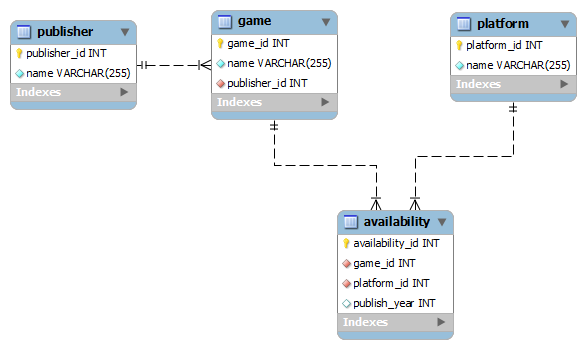
\includegraphics[scale=0.75]{videoGameDatabase}
\caption{Video Game Database Entity-Relation Diagram}
\label{figure:videoGameDatabase}
\end{figure}
 
This is a well-designed database with well-defined relationships 
between data records.  Data is not duplicated as it would be if 
we stored all of this information in a flat file.  Moreover, the 
integrity of the data is enforced by its design:
\begin{itemize}
  \item A publisher can exist independent of any game or platform 
  	records in our database, however
  \item A game cannot exist without a publisher--that is, the proper 
	publisher record must be present in the database before we 
	can insert a game and we must make a proper reference back 
	to the proper publisher record (through the use of foreign and 
	primary keys).
  \item A platform and a game can exist independent of each other.  
	It is only when we insert a record into the availability table that 
	those records are brought together and a relationship is defined.  
	However, the game and platform records need to exist before 
	we can define that relation.
\end{itemize}
	
We will not go into the details of how this database was designed, 
built and implemented using SQL (Structured Query Language).  
Instead, the focus of this lab will be to use an API (Application 
Programmer Interface) that we've built for you.

\subsection*{ODBC and the Database API}

An RDMS is used for the storage of data.  There are many vendors 
and database systems available (MSSQL, MySQL, PostgreSQL, 
Oracle, etc.).  Some of these are free and open source, others are 
``freeware'' and others cost millions of dollars.  If programs were 
written specifically to connect to only one of these databases, then 
we would need to rewrite the application if we ever wanted to 
migrate to a different RDMS (if we wanted to move to a cheaper 
alternative or if we needed to scale our application up to a larger, 
faster database system).  

Instead, applications are usually written on top of an abstract data 
access layer API which defines a general interface for interacting 
with a database.  Venders (Oracle, Microsoft) then publish drivers 
for these that provide specialized behavior for specific database 
systems.  The API that we'll be using for this lab is ODBC (Open 
DataBase Connectivity).  ODBC defines structures and functions 
that can be used to connect to a database, formulate queries (to 
insert, update, delete and select data) and process the results.  
Again, the details are beyond the scope of this lab; instead we 
have developed a small API that allows you to insert and retrieve 
data from the Video Game database described above.  

\section{Activities}

Clone the project code for this lab from GitHub using the following
URL: \url{https://github.com/cbourke/CSCE155-C-Lab15}.

\subsection{Viewing the Data}

Included in the project code are several source files that provide basic 
database functionality and definitions of structures that model games, 
publishers, and platforms.  Also included is a makefile to build all of the 
programs. 

\subsubsection*{Instructions}

\begin{enumerate}
  \item Open the \mintinline{text}{databaseInfo.h} header file and fill in values
  	for the \mintinline{c}{database} and \mintinline{c}{userId} variables and
	the \mintinline{c}{password} variables.  These
	credentials will be provided by your lab instructor.
  \item Open the \mintinline{text}{listGames.c} source file and look 
	at the code.  Build this program by executing the following from the 
	command line: \mintinline{text}{make listGames}
  \item Run the demo that was built for you \mintinline{text}{./listGames} 
  	and observe the results.  We'll reuse this program later, so don't 
	make any changes to \mintinline{text}{listGames.c}.
  \item Now look at the source code contained in \mintinline{text}{games.h} 
	and \mintinline{text}{games.c} and answer the questions in your worksheet.
\end{enumerate}

\subsection{Inserting New Records}

In this activity, you will use our API to add your favorite video game to 
the database.  Note: every student in this lab (and in the other labs for 
this course) is working on the same database.  It is not likely that any 
individual student could break the database, but you should be aware 
that inserting the same video game/publisher/platform for which a 
record already exists will have no effect.  Though you are encouraged 
to enter your favorite game, if it is popular enough, someone else may 
have already inserted it.  If adding a game fails, try again with another 
title (you may make one up if you need to).

\subsubsection*{Instructions}

Edit the \mintinline{text}{insertGame.c} source file and add code to add 
your favorite game to the database using our API.  To properly insert 
a new video game you need its name, the name of its publisher, at 
least one platform that it has been published on and its published year.

\begin{enumerate}
  \item Use the \mintinline{c}{getGame} function to see if the game 
	already exists (this function returns a struct representing the game 
	or \mintinline{c}{NULL} if it is not in the database).  If the game 
	already exists the program should end and you should rerun it with 
	another game or a renamed game as described above.
  \item Use the \mintinline{c}{getPlatform} and \mintinline{c}{getPublisher} 
	functions to find records (if they exist) for the platform and publisher 
	of your game.  If records do not exist (the functions return 
	\mintinline{c}{NULL}) then use the \mintinline{c}{addPlatform} and 
	\mintinline{c}{addPublisher} functions to add them first.
  \item Compile and run your program using
	
	\begin{minted}{text}
	make insertGame
	./insertGame
	\end{minted}
  \item Run the \mintinline{text}{listGames} program from activity 1 
  	to verify that your program worked.  Show your code and demonstrate 
	this to a lab instructor.
\end{enumerate}

\subsection{Ensuring Data Integrity}

Relational databases are intended to enforce constraints and ensure 
good data integrity.  In this activity you'll see what happens when those
constraints are violated.

\begin{enumerate}
  \item Attempt to add a game in an invalid publisher id and see what 
  	error(s) result.  Write a program to execute the following:
	
	\begin{minted}{c}
	addVideoGame("Pac Man's Revenge", 12345678, sqlstatementhandle);
	extractError("", sqlstatementhandle, SQL_HANDLE_STMT);
	\end{minted}
  \item Run the program and answer the questions on your worksheet.
\end{enumerate}

\section{Advanced Activity (optional)}

Contrast the code in the \mintinline{c}{addGame} and 
\mintinline{c}{addPublisher} functions.  The \mintinline{c}{addGame} 
function uses what is known as a prepared statement: a statement 
that has parameters (denoted with a question mark) and uses the 
API to prepare the statement and set those parameters.  The 
\mintinline{c}{addPublisher} function does not use parameters, but 
directly places the value of each column directly into the string.  
Prepared statements are the preferred way of doing database 
queries especially with applications that accept data entered by 
users.  Unprepared statements are susceptible to SQL Injection 
Attacks where a malicious user can inject their own SQL statements 
into the application's database calls and execute unauthorized 
SQL statements on the database.  Review the example and the 
documentation for ODBC and change the statements in the 
\mintinline{c}{addPublisher} and \mintinline{c}{addPlatform} 
functions to prepared statements.

	
\end{document}
